\documentclass[11pt,a4paper]{article}
\usepackage[utf8]{inputenc}
\usepackage[T1]{fontenc}
\usepackage{lmodern}
\usepackage[french]{babel}
\usepackage[a4paper,top=2.2cm,bottom=2.1cm,left=2.3cm,right=2.3cm]{geometry}
\usepackage{graphicx}
\usepackage{booktabs}
\usepackage{array}
\usepackage{xcolor}
\usepackage{tikz}
\usetikzlibrary{positioning,arrows.meta,shapes.geometric}
\usepackage{fancyhdr}
\usepackage{enumitem}
\usepackage[hidelinks]{hyperref}
\usepackage{caption}
\usepackage{float}

\definecolor{navy}{HTML}{123159}
\definecolor{accent}{HTML}{2E71E4}
\definecolor{soft}{HTML}{EEF3FB}

\setlength{\parindent}{0pt}
\setlength{\parskip}{6pt}
\setlist{itemsep=2pt,topsep=3pt}
\captionsetup{font=small,labelfont=bf}

\pagestyle{fancy}
\fancyhf{}
\fancyhead[L]{\small Projet 18 : Fraudes financi\`eres et cycles de blanchiment}
\fancyhead[R]{\small Groupe 4}
\fancyfoot[C]{\small\thepage}
\renewcommand{\headrulewidth}{0.3pt}

\begin{document}

%================ PAGE DE GARDE ================
\begin{titlepage}
\thispagestyle{empty}
\centering
\vspace*{1.2cm}
{\large Mini-projet Big Data n\textdegree 18 \quad|\quad Groupe 4}\\[2.2cm]
{\color{navy}\rule{\textwidth}{1.2pt}}\\[0.6cm]
{\Huge\bfseries\color{navy} D\'etection en temps r\'eel\\ de fraudes financi\`eres,\\[4pt] analyse de r\'eseaux suspects\\[4pt] et d\'ecouverte de cycles\\ de blanchiment\par}
\vspace{0.6cm}
{\color{navy}\rule{\textwidth}{1.2pt}}\\[1.0cm]
{\Large GraphFrames \;+\; Kafka \;+\; Delta Lake}\\[0.3cm]
{\large avec supervision Prometheus et Grafana}\\[3.2cm]
{\Large\bfseries Marouan Ezbakhe}\\[0.2cm]
{\Large\bfseries Mohammed Hamdouch}\\[2.6cm]
{\large Rapport de projet}\\[0.2cm]
{\large Novembre 2026}\\[1.6cm]
{\small D\'ep\^ot du code : \texttt{github.com/Marouan333/fraud-detection-big-data}}
\end{titlepage}

%================ RESUME + TABLE ================
\newpage
\begin{abstract}
\noindent Ce rapport pr\'esente un pipeline Big Data qui r\'epond \`a deux probl\`emes de criminalit\'e financi\`ere : d\'etecter la fraude au moment o\`u elle se produit, et r\'ev\'eler des circuits de blanchiment cach\'es dans un r\'eseau de comptes. La premi\`ere partie rejoue 6\,362\,620 transactions PaySim dans \textbf{Kafka}, les traite avec \textbf{Spark Structured Streaming} et les stocke dans \textbf{Delta Lake} avec une garantie d'\'ecriture sans doublon. La seconde partie construit un graphe de 515\,088 comptes et 5\,078\,345 transactions (IBM AML) et applique \textbf{GraphFrames} : PageRank pour rep\'erer les comptes pivots, Label Propagation pour les communaut\'es et composantes fortement connexes pour les cycles. L'ensemble est supervis\'e en direct avec \textbf{Prometheus} et \textbf{Grafana}. Les r\'esultats sont mesur\'es : un compte du top~1\,\% de PageRank a 4,2 fois plus de chances d'\^etre impliqu\'e dans du blanchiment qu'un compte pris au hasard, et 50 cycles couvrant 289 comptes sont identifi\'es.
\end{abstract}
\vspace{0.4cm}
{\color{navy}\rule{\textwidth}{0.6pt}}
\setcounter{tocdepth}{1}
\tableofcontents
\vspace{0.3cm}

%================ 1 INTRODUCTION ================
\section{Introduction}
\subsection{Contexte}
Les institutions financi\`eres traitent chaque jour des millions de transactions. Deux menaces se cachent dans ce volume. La \textbf{fraude} est visible dans une transaction isol\'ee : un virement inhabituel, un retrait imm\'ediat apr\`es un transfert. Le \textbf{blanchiment d'argent} ne se voit pas ligne par ligne : il appara\^it dans la \emph{structure} des \'echanges, quand l'argent traverse de nombreux comptes pour masquer son origine, parfois en revenant \`a son point de d\'epart.

Ces deux probl\`emes appellent deux familles d'outils. Le premier demande de traiter un flux continu avec une faible latence. Le second demande de raisonner sur un r\'eseau de relations.

\subsection{Objectifs}
Le sujet du projet est \og D\'etection en temps r\'eel de fraudes financi\`eres, analyse de r\'eseaux suspects et d\'ecouverte de cycles de blanchiment \fg{} avec GraphFrames, Kafka et Delta Lake. Nous l'avons d\'ecoup\'e en quatre objectifs :
\begin{enumerate}
  \item Ing\'erer en continu un flux de transactions avec Kafka et Spark Structured Streaming.
  \item Stocker les r\'esultats de fa\c{c}on fiable (ACID, sans doublon) dans Delta Lake.
  \item Analyser un graphe de transactions avec GraphFrames pour identifier des comptes suspects et des cycles.
  \item Superviser le pipeline en temps r\'eel avec Prometheus et Grafana, comme demand\'e par l'encadrant.
\end{enumerate}

\subsection{D\'emarche et organisation du rapport}
Nous avons construit le projet par \'etapes, en mesurant chaque r\'esultat. Les sections suivantes d\'ecrivent les donn\'ees (section~2), l'architecture (section~3), le streaming (section~4), la fiabilit\'e du stockage (section~5), la supervision (section~6), l'analyse de graphes (sections~7 et~8), les optimisations (section~9), puis les r\'esultats, limites et perspectives (section~10).

%================ 2 DONNEES ================
\section{Les jeux de donn\'ees}
Nous utilisons deux jeux de donn\'ees publics, chacun associ\'e \`a une moiti\'e du projet.

\subsection{PaySim : le flux temps r\'eel}
PaySim simule des transactions de monnaie mobile. Il contient \textbf{6\,362\,620} transactions dont \textbf{8\,213} frauduleuses (0,13\,\%). Les colonnes utilis\'ees sont : \texttt{step} (heure simul\'ee), \texttt{type} (PAYMENT, CASH\_OUT, CASH\_IN, TRANSFER, DEBIT), \texttt{amount}, \texttt{nameOrig} (\'emetteur), \texttt{nameDest} (destinataire) et \texttt{isFraud} (\'etiquette). Ce jeu est envoy\'e transaction par transaction dans Kafka pour simuler un flux r\'eel.

\subsection{IBM AML HI-Small : le graphe}
Ce jeu contient \textbf{5\,078\,345} transactions entre \textbf{515\,088} comptes, dont \textbf{5\,177} marqu\'ees comme blanchiment (0,10\,\%). Nous en faisons un graphe orient\'e : un \textbf{n\oe ud} est un compte, une \textbf{ar\^ete} est une transaction. Un compte est identifi\'e par \texttt{banque\_compte}, car un m\^eme num\'ero peut exister dans deux banques diff\'erentes et ne doit pas \^etre fusionn\'e.

\begin{figure}[H]
\centering
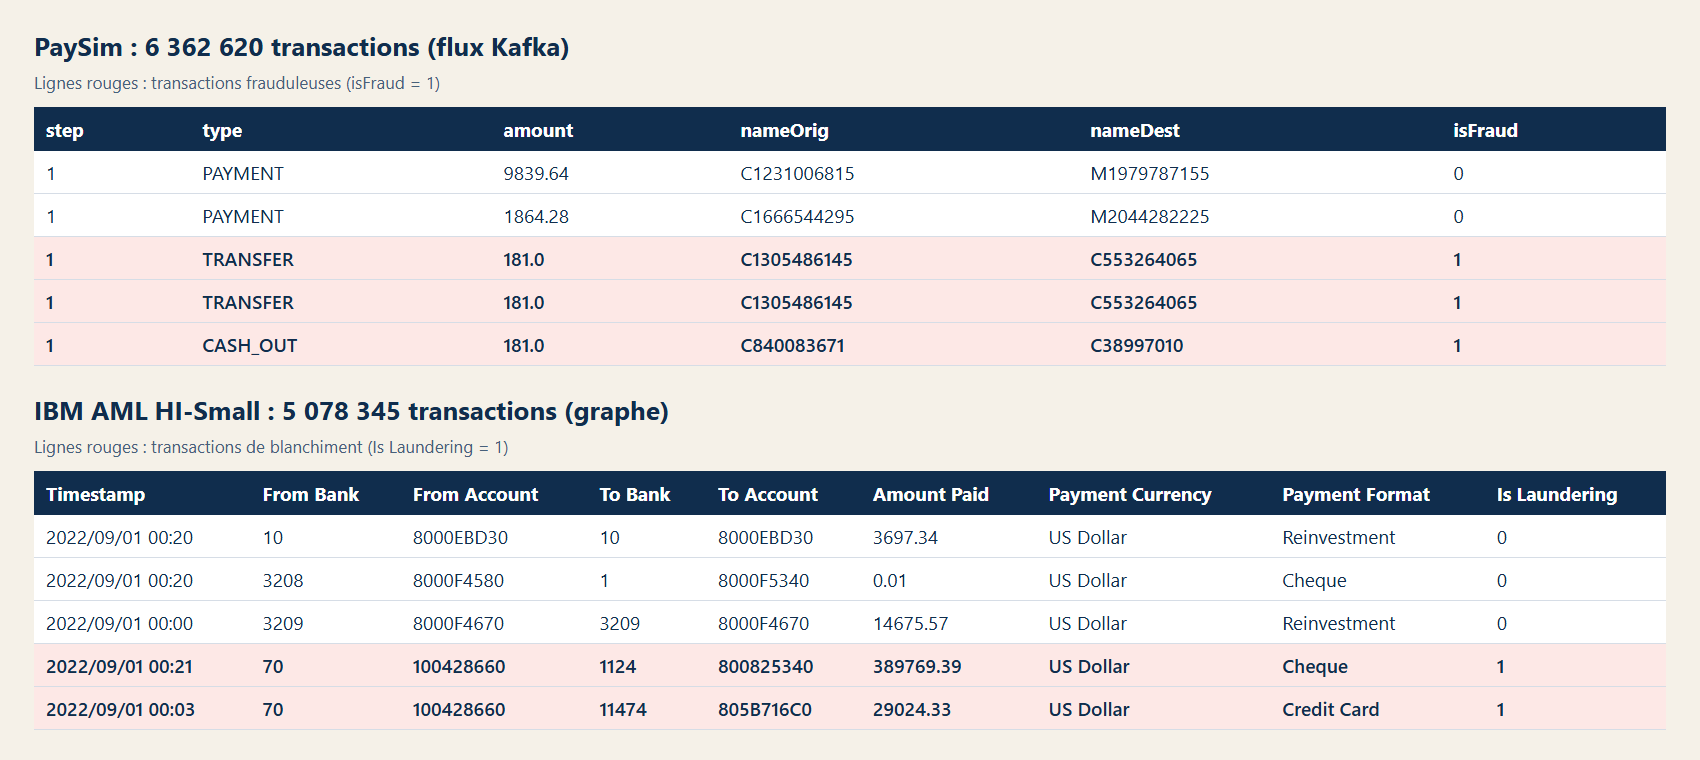
\includegraphics[width=0.98\textwidth]{figures/datasets.png}
\caption{\'Echantillon r\'eel des deux fichiers. Les lignes roses sont des cas positifs (fraude ou blanchiment).}
\end{figure}

\subsection{Un d\'es\'equilibre extr\^eme}
Dans les deux jeux, moins de 0,15\,\% des lignes sont des cas positifs. Cons\'equence directe : la pr\'ecision globale ne mesure rien (un mod\`ele qui r\'epond toujours \og normal \fg{} a raison 99,9\,\% du temps). Nous mesurons donc la \emph{pr\'ecision}, le \emph{rappel} et le \emph{lift} par rapport au hasard.

\begin{figure}[H]
\centering
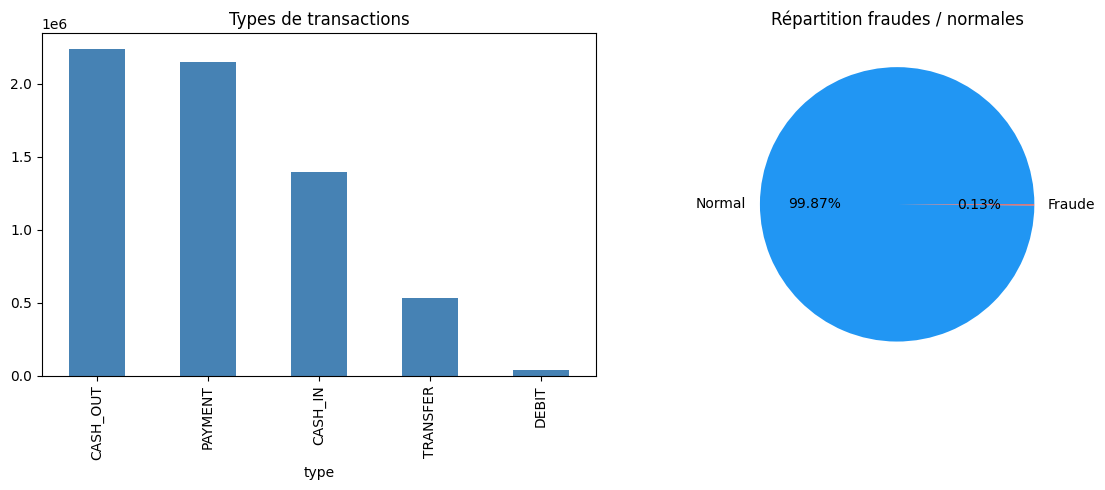
\includegraphics[width=0.62\textwidth]{figures/paysim_explo.png}
\caption{Exploration de PaySim : types de transactions et part de fraude.}
\end{figure}

%================ 3 ARCHITECTURE ================
\section{Architecture et technologies}
Le projet comporte deux cha\^ines qui partagent le m\^eme stockage et la m\^eme supervision (figure~\ref{fig:archi}).

\begin{figure}[H]
\centering
\begin{tikzpicture}[
  box/.style={draw=navy,fill=soft,rounded corners=3pt,minimum height=0.95cm,minimum width=2.15cm,align=center,font=\small},
  big/.style={draw=navy,fill=navy,text=white,rounded corners=3pt,minimum height=2.1cm,minimum width=2.2cm,align=center,font=\bfseries\small},
  mon/.style={draw=accent,fill=white,rounded corners=3pt,minimum height=0.95cm,minimum width=2.6cm,align=center,font=\small},
  arr/.style={-{Stealth[length=2.2mm]},thick,navy}]
\node[box] (ps) {PaySim\\ \scriptsize 6,36 M tx};
\node[box,right=0.45cm of ps] (kf) {Kafka};
\node[box,right=0.45cm of kf] (sp) {Spark\\ \scriptsize Streaming};
\node[big,right=0.7cm of sp] (dl) {Delta\\ Lake};
\node[box,below=1.15cm of ps] (ib) {IBM AML\\ \scriptsize 5,08 M tx};
\node[box,right=0.45cm of ib,minimum width=4.9cm] (gf) {GraphFrames\\ \scriptsize PageRank, Label Prop., SCC};
\node[mon,below=0.7cm of dl,xshift=2.2cm] (gr) {Prometheus\\ + Grafana};
\draw[arr] (ps)--(kf); \draw[arr] (kf)--(sp); \draw[arr] (sp)--(dl);
\draw[arr] (ib)--(gf); \draw[arr] (gf.east)-|(dl.south);
\draw[arr,accent,dashed] (dl.east)-|(gr.north);
\end{tikzpicture}
\caption{Architecture globale : un flux temps r\'eel (haut), un traitement de graphe (bas), un stockage commun et une supervision.}
\label{fig:archi}
\end{figure}

\begin{center}
\small
\begin{tabular}{@{}p{3.2cm}p{5.4cm}p{5.2cm}@{}}
\toprule
\textbf{Technologie} & \textbf{R\^ole} & \textbf{O\`u dans le projet} \\
\midrule
Kafka et Zookeeper & Bus de messages qui re\c{c}oit les transactions & \texttt{docker-compose.yml}, \texttt{producer/} \\
Spark Structured Streaming & Lecture de Kafka par micro-batch & \texttt{streaming/spark\_consumer.py} \\
Delta Lake & Stockage ACID, historique, compaction & dossier \texttt{delta\_lake/} \\
GraphFrames & PageRank, Label Propagation, SCC & \texttt{graph/} \\
Prometheus et Grafana & M\'etriques et tableau de bord & \texttt{monitoring/} \\
Docker Compose & Lance Kafka, Zookeeper, Prometheus, Grafana & \texttt{docker-compose.yml} \\
\bottomrule
\end{tabular}
\end{center}

Les services Docker disposent de \emph{health checks} : Kafka ne d\'emarre qu'une fois Zookeeper pr\^et, et red\'emarre seul en cas d'\'echec. Sans cela, Kafka s'arr\^etait au d\'emarrage lorsqu'il n'atteignait pas Zookeeper \`a temps.

%================ 4 STREAMING ================
\section{Le pipeline de streaming}
\subsection{Le producteur Kafka}
Le producteur (\texttt{producer/kafka\_producer.py}) lit le fichier PaySim \emph{par blocs de 100\,000 lignes} et seulement les six colonnes utiles, ce qui borne la m\'emoire. Chaque transaction est envoy\'ee en JSON avec un identifiant unique \texttt{tx\_id}. L'envoi se fait par lots compress\'es (gzip, d\'elai de regroupement de 20\,ms, lots de 256\,Ko) et la cl\'e de partition est le compte \'emetteur, ce qui conserve l'ordre des transactions d'un m\^eme compte. Sur le jeu complet, le producteur envoie \textbf{6\,362\,620 messages en 1\,765\,s}, soit environ 3\,600 transactions par seconde (5\,000 au d\'ebut, avant que Spark ne partage le processeur de la machine).

\subsection{Kafka}
Kafka est un journal de messages. Le producteur \'ecrit dans un \emph{topic}, chaque message re\c{c}oit un \emph{offset} (sa position) et plusieurs consommateurs peuvent le relire. Il d\'ecouple l'\'emetteur du lecteur : si Spark est lent ou arr\^et\'e, aucun message n'est perdu. Le topic est cr\'e\'e automatiquement s'il n'existe pas, ce qui permet de d\'emarrer producteur et consommateur dans n'importe quel ordre.

\subsection{Le consommateur Spark Structured Streaming}
Le consommateur (\texttt{streaming/spark\_consumer.py}) lit Kafka par \textbf{micro-batch toutes les 10 secondes}, au plus 200\,000 messages par batch. La fonction \texttt{foreachBatch} permet, pour chaque batch, d'\'ecrire toutes les transactions dans une table Delta, d'isoler les fraudes dans une seconde table et de mettre \`a jour les compteurs Prometheus. Le batch est mis en cache : Kafka est lu et le JSON analys\'e une seule fois au lieu de quatre.

\begin{figure}[H]
\centering
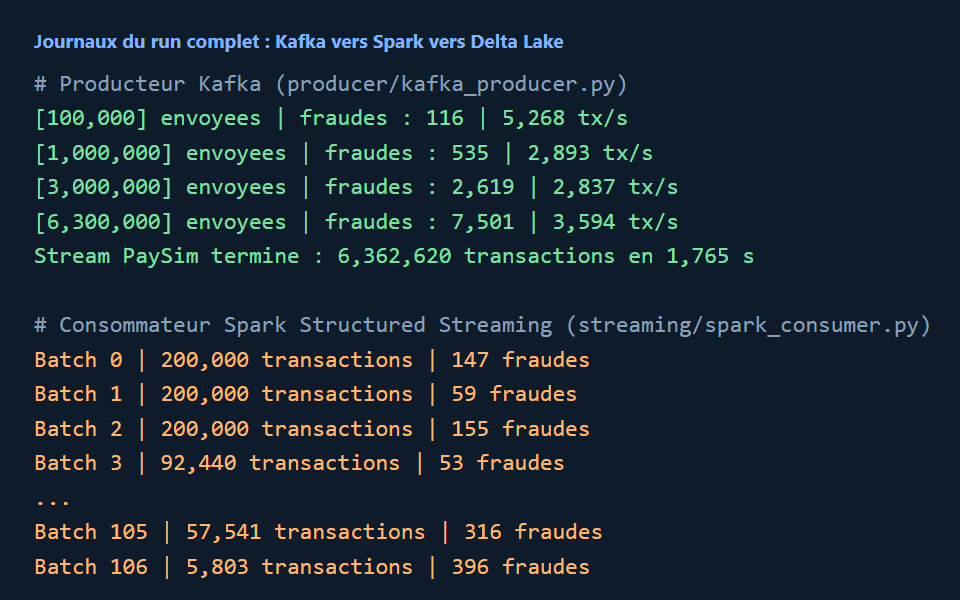
\includegraphics[width=0.58\textwidth]{figures/logs.png}
\caption{Journaux r\'eels du run complet : producteur Kafka (haut) et consommateur Spark (bas).}
\end{figure}

\subsection{Garantie \og exactement une fois \fg}
Deux m\'ecanismes se combinent :
\begin{itemize}
  \item le \textbf{checkpoint} m\'emorise les offsets Kafka d\'ej\`a trait\'es : apr\`es un red\'emarrage, Spark reprend o\`u il s'\'etait arr\^et\'e ;
  \item les \'ecritures Delta portent \texttt{txnAppId} et \texttt{txnVersion} (le num\'ero de batch) : si Spark rejoue un batch, Delta ignore l'\'ecriture d\'ej\`a valid\'ee.
\end{itemize}

%================ 5 DELTA ================
\section{Delta Lake et fiabilit\'e du stockage}
Delta Lake ajoute \`a des fichiers Parquet un journal de transactions. Il apporte des \'ecritures atomiques (ACID), l'historique des versions (\emph{time travel}) et des lectures coh\'erentes pendant que le streaming \'ecrit. Le projet produit cinq tables :

\begin{center}
\small
\begin{tabular}{@{}lp{9.5cm}@{}}
\toprule
\textbf{Table} & \textbf{Contenu} \\
\midrule
\texttt{transactions} & toutes les transactions ing\'er\'ees (6\,362\,620 lignes) \\
\texttt{fraud\_alerts} & transactions marqu\'ees frauduleuses (8\,213 lignes) \\
\texttt{suspicious\_nodes} & comptes suspects selon PageRank (top 1\,\%) \\
\texttt{cycle\_nodes} & comptes appartenant \`a un cycle \\
\texttt{laundering\_cycles} & transactions de blanchiment au sein des cycles \\
\bottomrule
\end{tabular}
\end{center}

\subsection{Un probl\`eme de doublons, trouv\'e puis corrig\'e}
Lors des premiers tests, la table \texttt{transactions} contenait \textbf{8\,121\,085} lignes pour seulement 6\,362\,620 transactions r\'eelles. La cause : sans checkpoint, chaque red\'emarrage du consommateur relisait le topic Kafka depuis le d\'ebut. Nous avons corrig\'e le code (checkpoint et \'ecritures idempotentes, section~4) puis nettoy\'e la table. Un test de contr\^ole a confirm\'e le r\'esultat : consommateur arr\^et\'e puis relanc\'e, 50\,000 lignes attendues, 50\,000 lignes obtenues, aucune en double.

\subsection{Maintenance}
Le streaming \'ecrit un petit fichier par batch : 348 fichiers pour la table \texttt{transactions}. Le script \texttt{maintenance/optimize\_delta.py} d\'edoublonne sur la cl\'e m\'etier et compacte ces fichiers en 3, sans supprimer l'historique (pas de \texttt{VACUUM}). Apr\`es maintenance, la table contient exactement 6\,362\,620 lignes, sans doublon.

%================ 6 SUPERVISION ================
\section{Supervision avec Prometheus et Grafana}
La supervision en direct est une exigence du projet. Elle fonctionne en trois \'etapes :
\begin{enumerate}
  \item \textbf{Exposition.} Le producteur (port 8000) et le consommateur (port 8001) publient des compteurs avec la biblioth\`eque \texttt{prometheus\_client}.
  \item \textbf{Collecte.} Prometheus visite ces deux adresses toutes les 5 secondes et enregistre les valeurs avec leur horodatage (\texttt{monitoring/prometheus.yml}).
  \item \textbf{Affichage.} Grafana interroge Prometheus et dessine les panneaux. Le tableau de bord est provisionn\'e automatiquement au d\'emarrage (\texttt{monitoring/grafana\_dashboard.json}).
\end{enumerate}

\begin{center}
\small
\begin{tabular}{@{}lp{8.6cm}@{}}
\toprule
\textbf{Compteur} & \textbf{Signification} \\
\midrule
\texttt{producer\_transactions\_total} & transactions envoy\'ees \`a Kafka \\
\texttt{producer\_fraud\_total} & fraudes parmi les transactions envoy\'ees \\
\texttt{consumer\_transactions\_total} & transactions ing\'er\'ees par Spark \\
\texttt{consumer\_fraud\_detected\_total} & fraudes isol\'ees par Spark \\
\texttt{consumer\_batches\_total} & micro-batchs trait\'es \\
\bottomrule
\end{tabular}
\end{center}

\begin{figure}[H]
\centering
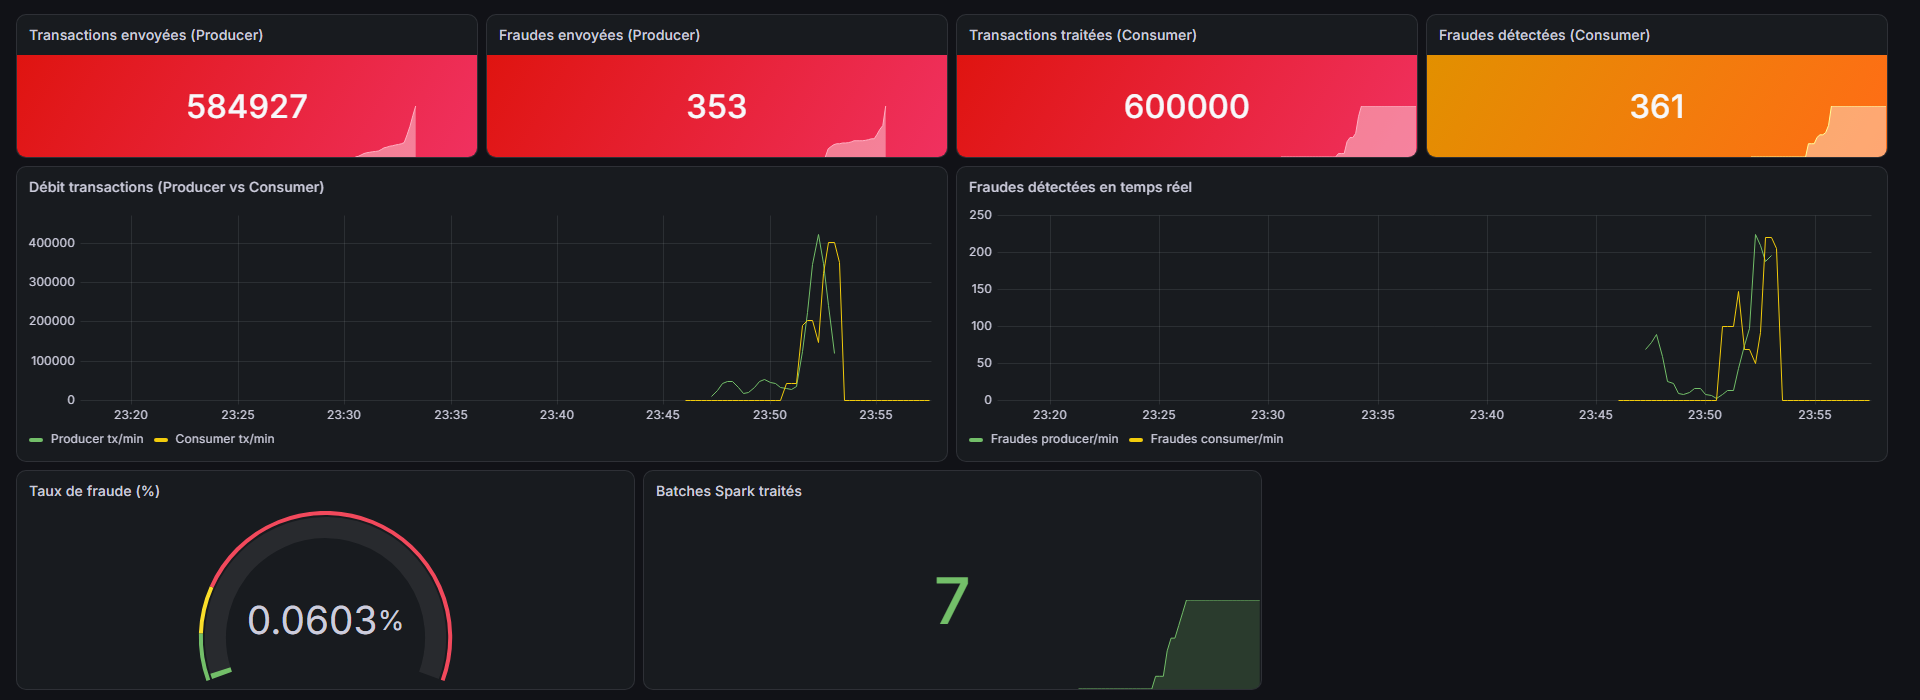
\includegraphics[width=0.98\textwidth]{figures/grafana.png}
\caption{Tableau de bord Grafana r\'eel pendant un run de 600\,000 transactions : 600\,000 trait\'ees, 361 fraudes d\'etect\'ees, 7 batchs Spark.}
\end{figure}

Sur la capture, le producteur affiche 584\,927 transactions alors que 600\,000 ont \'et\'e trait\'ees. Ce n'est pas une perte : le producteur s'est arr\^et\'e avant la derni\`ere lecture de Prometheus, qui conserve la derni\`ere valeur lue.

%================ 7 GRAPHE ================
\section{Analyse de graphes : comptes suspects}
\subsection{Construction du graphe}
Le fichier IBM AML est lu avec un \emph{sch\'ema explicite} (sans inf\'erence de types), ce qui \'evite une passe compl\`ete sur 5 millions de lignes et nomme proprement les deux colonnes \og Account \fg{} dupliqu\'ees dans l'en-t\^ete. Les n\oe uds sont les identifiants \texttt{banque\_compte}, les ar\^etes les transactions avec leur montant, leur devise et leur format de paiement.

\begin{figure}[H]
\centering
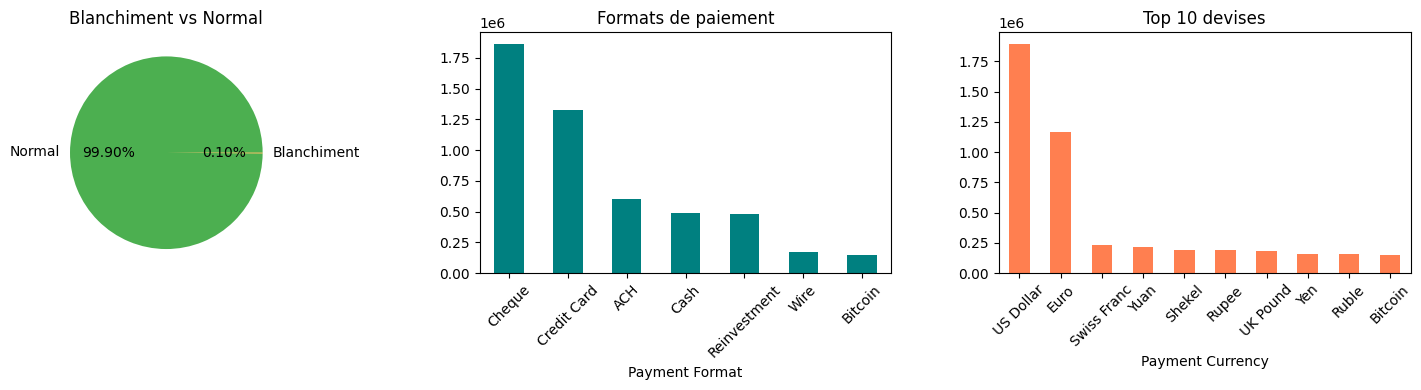
\includegraphics[width=0.85\textwidth]{figures/aml_explo.png}
\caption{Exploration du jeu IBM AML : part de blanchiment, formats de paiement et devises.}
\end{figure}

\subsection{PageRank}
PageRank, \`a l'origine l'algorithme de classement de Google, attribue un score \'elev\'e \`a un compte qui re\c{c}oit des flux de comptes eux-m\^emes importants. Les scores ont une moyenne de 1. Notre premier seuil, \og score sup\'erieur \`a 1,0 \fg{}, retenait 201\,950 comptes (environ 40\,\%), ce qui est inutilisable. Nous avons remplac\'e ce seuil par le \textbf{percentile 99} des scores (6,21), soit \textbf{5\,189 comptes}, et nous les confrontons aux 6\,357 comptes de blanchiment connus.

\begin{center}
\small
\begin{tabular}{@{}lr@{}}
\toprule
\textbf{Indicateur} & \textbf{Valeur} \\
\midrule
Comptes analys\'es & 515\,088 \\
Comptes retenus (top 1\,\%) & 5\,189 \\
Dont r\'eellement impliqu\'es dans du blanchiment & 267 \\
Pr\'ecision & 5,15\,\% \\
Taux de base (tirage au hasard) & 1,23\,\% \\
\textbf{Lift} & \textbf{4,2} \\
Rappel & 4,2\,\% \\
\bottomrule
\end{tabular}
\end{center}

Un compte du top 1\,\% a donc 4,2 fois plus de chances d'\^etre impliqu\'e dans du blanchiment qu'un compte pris au hasard. Le rappel reste faible : PageRank rep\`ere les comptes pivots, alors qu'une grande partie du blanchiment passe par des comptes peu connect\'es.

\begin{figure}[H]
\centering
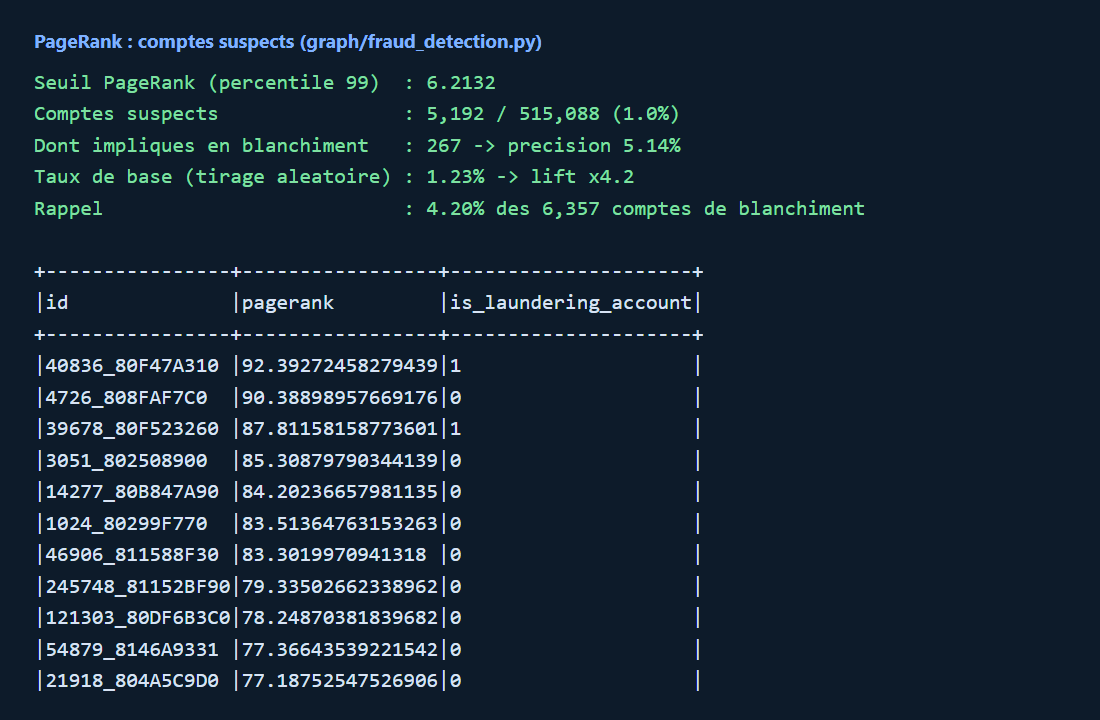
\includegraphics[width=0.5\textwidth]{figures/pagerank.png}
\caption{Sortie r\'eelle du script \texttt{fraud\_detection.py}. Les comptes n\textdegree 1 et n\textdegree 3 sont de vrais comptes de blanchiment (colonne de droite).}
\end{figure}

\subsection{Label Propagation}
Chaque compte adopte l'\'etiquette la plus fr\'equente parmi ses voisins ; les groupes densement connect\'es convergent vers une m\^eme \'etiquette et forment des communaut\'es. La plus grande regroupe 6\,654 comptes.

%================ 8 CYCLES ================
\section{D\'ecouverte de cycles de blanchiment}
Une \textbf{composante fortement connexe} (SCC) est un ensemble de comptes dans lequel chaque compte peut atteindre tous les autres en suivant le sens de l'argent : l'argent peut donc revenir \`a son point de d\'epart, signature classique du blanchiment.

Lancer l'algorithme sur les 5 millions d'ar\^etes saturait la m\'emoire du driver (plus de 140\,000 \'etapes Spark, \texttt{OutOfMemoryError}). Nous l'ex\'ecutons donc sur le \textbf{sous-graphe de blanchiment} : 5\,177 ar\^etes et 6\,357 n\oe uds. Le calcul se termine alors en quelques minutes.

\begin{center}
\small
\begin{tabular}{@{}lr@{}}
\toprule
\textbf{Indicateur} & \textbf{Valeur} \\
\midrule
Cycles d\'etect\'es (composantes de taille $>1$) & 50 \\
Comptes impliqu\'es dans ces cycles & 289 \\
Transactions de blanchiment dans les cycles & 585 \\
Plus grand cycle & 25 comptes \\
\bottomrule
\end{tabular}
\end{center}

\begin{figure}[H]
\centering
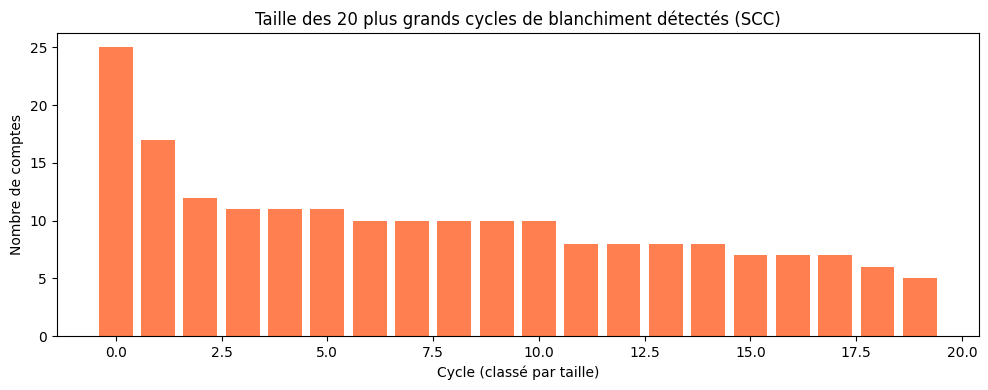
\includegraphics[width=0.68\textwidth]{figures/cycles.png}
\caption{Taille des 20 plus grands cycles de blanchiment d\'etect\'es.}
\end{figure}

\textbf{Limite assum\'ee.} Ce sous-graphe est s\'electionn\'e gr\^ace \`a l'\'etiquette de blanchiment : cette \'etape d\'ecrit donc la structure du blanchiment connu plut\^ot qu'elle ne d\'ecouvre des cas inconnus. En production, on l'appliquerait au voisinage des comptes suspects remont\'es par PageRank.

%================ 9 OPTIMISATIONS ================
\section{Optimisations d'ing\'enierie}
Apr\`es une premi\`ere version fonctionnelle, nous avons audit\'e et am\'elior\'e le pipeline :
\begin{itemize}
  \item \textbf{Fiabilit\'e :} checkpoint Kafka et \'ecritures Delta idempotentes (fin des doublons).
  \item \textbf{Producteur :} lecture par blocs, lots compress\'es, cl\'e de partition, \texttt{tx\_id} unique ; d\'ebit mesur\'e d'environ 5\,000 tx/s au lieu de 100 \`a 170 avec \texttt{iterrows()}.
  \item \textbf{Consommateur :} un seul calcul par batch (cache), contre-pression avec \texttt{maxOffsetsPerTrigger}.
  \item \textbf{Graphe :} sch\'ema explicite, chargement partag\'e entre les scripts, un sous-graphe pour SCC.
  \item \textbf{Spark :} une seule configuration centralis\'ee (m\'emoire, Adaptive Query Execution, JAR).
  \item \textbf{Infrastructure :} \emph{health checks} Docker, variables d'environnement pour tester sans toucher aux donn\'ees r\'eelles.
  \item \textbf{Maintenance :} d\'edoublonnage et compaction Delta (348 fichiers en 3).
\end{itemize}

%================ 10 RESULTATS ================
\section{R\'esultats, limites et perspectives}
\subsection{Synth\`ese des r\'esultats}
\begin{center}
\small
\begin{tabular}{@{}p{8.2cm}r@{}}
\toprule
\textbf{R\'esultat mesur\'e} & \textbf{Valeur} \\
\midrule
Transactions ing\'er\'ees dans Delta Lake (aucun doublon) & 6\,362\,620 \\
Fraudes isol\'ees dans \texttt{fraud\_alerts} & 8\,213 \\
Dur\'ee du streaming complet & 1\,765\,s \\
Comptes suspects (top 1\,\% PageRank) / lift & 5\,189 / 4,2 \\
Cycles de blanchiment / comptes / transactions & 50 / 289 / 585 \\
\bottomrule
\end{tabular}
\end{center}

\subsection{Limites}
\begin{itemize}
  \item La d\'etection en streaming s'appuie sur l'\'etiquette \texttt{isFraud} de PaySim : elle d\'emontre le pipeline (ingestion, stockage, supervision \`a grande \'echelle), mais ce n'est pas un mod\`ele appris.
  \item Le rappel de PageRank est de 4,2\,\% : il rep\`ere les pivots, pas les comptes peu connect\'es.
  \item L'analyse des cycles porte sur le sous-graphe de blanchiment connu (section~8).
  \item Le d\'ebit de 3\,600 tx/s est limit\'e par une machine unique qui h\'eberge Kafka, Spark et les scripts.
\end{itemize}

\subsection{Perspectives}
Le sujet n'impose pas de mod\`ele d'apprentissage, mais le pipeline s'y pr\^ete : un mod\`ele entra\^in\'e sur l'historique pourrait noter chaque batch. Une couche \og bronze \fg{} en Parquet acc\'el\'ererait les relances des jobs de graphe, et le m\^eme code s'ex\'ecuterait sur un cluster Spark en changeant seulement le param\`etre \texttt{SPARK\_MASTER}. Enfin, appliquer l'analyse de cycles au voisinage des comptes suspects de PageRank la rendrait utile pour des cas inconnus.

\subsection{Conclusion}
Le projet r\'epond aux trois volets du sujet avec les technologies demand\'ees : \emph{temps r\'eel} (Kafka et Spark Streaming), \emph{r\'eseaux suspects} (PageRank et Label Propagation) et \emph{cycles de blanchiment} (composantes fortement connexes avec GraphFrames), le tout stock\'e dans Delta Lake et supervis\'e par Prometheus et Grafana. Les r\'esultats sont mesur\'es et reproductibles : le code, la documentation et la proc\'edure d'ex\'ecution sont disponibles sur le d\'ep\^ot GitHub du projet.

\subsection{R\'epartition de la pr\'esentation}
\textbf{Marouan Ezbakhe} : architecture, streaming Kafka et Spark, jeux de donn\'ees, supervision. \textbf{Mohammed Hamdouch} : graphe IBM AML, PageRank et communaut\'es, cycles, conclusion.

\end{document}
